\tableofcontents

\newpage

\section{Задание}
По выданному преподавателем варианту разработать программу асинхронного обмена данными с внешним устройством. При помощи программы осуществить ввод или вывод информации, используя в качестве подтверждения данных сигнал (кнопку) готовности ВУ.
\begin{figure}[H]
\centering
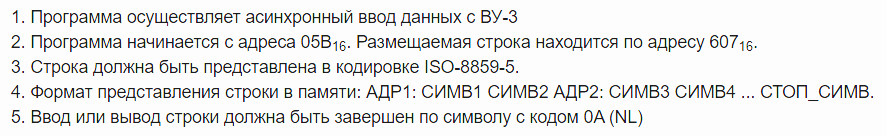
\includegraphics[scale=0.6]{task}
\label{pic:task}
\end{figure}

\section{Текст программы}
\begin{center}
\begin{tabular}{c}
\begin{lstlisting}[basicstyle=\ttfamily]
	ORG	0x213
ADDR:	WORD	$STRING
NOW:	WORD	0
NL:	WORD	0x0A
CFW:	WORD	0xFF
START:	LD	ADDR
	ST	NOW
NEXT:	CLA
S1:	IN	0x3
	AND	#0x40
	BEQ	S1
	LD	(NOW)
	SWAB
	AND	CFW
	CMP	NL
	OUT 	0x2
	BEQ	STOP
	CLA
S2:	IN	0x3
	AND	#0x40
	BEQ	S2
	LD	(NOW)+
	AND	CFW
	CMP	NL
	OUT	0x2
	BNE	NEXT
STOP:	HLT
	ORG	0x5D8
STRING:	WORD	0xBCEB
	WORD	0x0A00
\end{lstlisting}
\end{tabular}
\end{center}

\section{Вводимая строка}
\begin{center}
\begin{tabular}{|c|c|c|c|}
\hline
 & ISO-8859-5 & UTF-8 & UTF-16BE\\
\hline
М & BC & D0 9C & 04 1C\\
ы & EB & D1 8B & 04 4B\\
& 20 & 20 & 00 20\\
р & E0 & D1 80 & 04 40\\
а & D0 & D0 B0 & 04 30\\
б & D1 & D0 B1 & 04 31\\
о & DE & D0 BE & 04 3E\\
т & E2 & D1 82 & 04 42\\
а & D0 & D0 B0 & 04 30\\
е & D5 & D0 B5 & 04 35\\
м & DC & D0 BC & 04 3C\\
& 20 & 20 & 00 20\\
н & DD & D0 BD & 04 3D\\
а & D0 & D0 B0 & 04 30\\
д & D4 & D0 B4 & 04 34\\
& 20 & 20 & 00 20\\
э & ED & D1 8D & 04 4D\\
т & E2 & D1 82 & 04 42\\
и & D8 & D0 B8 & 04 38\\
м & DC & D0 BC & 04 3C\\
& 20 & 20 & 00 20\\
- & 2D & 2D & 00 2D\\
& 20 & 20 & 00 20\\
ф & E4 & D1 84 & 04 44\\
р & E0 & D1 80 & 04 40\\
а & D0 & D0 B0 & 04 30\\
з & D7 & D0 B7 & 04 37\\
а & D0 & D0 B0 & 04 30\\
- & 2D & 2D & 00 2D\\
з & D7 & D0 B7 & 04 37\\
а & D0 & D0 B0 & 04 30\\
в & D2 & D0 B2 & 04 32\\
т & E2 & D1 82 & 04 42\\
р & E0 & D1 80 & 04 40\\
а & D0 & D0 B0 & 04 30\\
к & DA & D0 BA & 04 3A\\
, & 2C & 2C & 00 2C\\
& 20 & 20 & 00 20\\
к & DA & D0 BA & 04 3A\\
о & DE & D0 BE & 04 3E\\
т & E2 & D1 82 & 04 42\\
о & DE & D0 BE & 04 3E\\
р & E0 & D1 80 & 04 40\\
ы & EB & D1 8B & 04 4B\\
м & DC & D0 BC & 04 3C\\
& 20 & 20 & 00 20\\
в & D2 & D0 B2 & 04 32\\
& 20 & 20 & 00 20\\
9 & 39 & 39 & 00 39\\
5 & 35 & 35 & 00 35\\
\% & 25 & 25 & 00 25\\
& 20 & 20 & 00 20\\
с & E1 & D1 81 & 04 41\\
л & DB & D0 BB & 04 3B\\
у & E3 & D1 83 & 04 43\\
ч & E7 & D1 87 & 04 47\\
а & D0 & D0 B0 & 04 30\\
\hline
\end{tabular}
\quad
\begin{tabular}{|c|c|c|c|}
\hline
 & ISO-8859-5 & UTF-8 & UTF-16BE\\
\hline
е & D5 & D0 B5 & 04 35\\
в & D2 & D0 B2 & 04 32\\
& 20 & 20 & 00 20\\
к & DA & D0 BA & 04 3A\\
о & DE & D0 BE & 04 3E\\
р & E0 & D1 80 & 04 40\\
м & DC & D0 BC & 04 3C\\
я & EF & D1 8F & 04 4F\\
т & E2 & D1 82 & 04 42\\
& 20 & 20 & 00 20\\
л & DB & D0 BB & 04 3B\\
ю & EE & D1 8E & 04 4E\\
д & D4 & D0 B4 & 04 34\\
е & D5 & D0 B5 & 04 35\\
й & D9 & D0 B9 & 04 39\\
, & 2C & 2C & 00 2C\\
& 20 & 20 & 00 20\\
к & DA & D0 BA & 04 3A\\
о & DE & D0 BE & 04 3E\\
т & E2 & D1 82 & 04 42\\
о & DE & D0 BE & 04 3E\\
р & E0 & D1 80 & 04 40\\
ы & EB & D1 8B & 04 4B\\
е & D5 & D0 B5 & 04 35\\
& 20 & 20 & 00 20\\
п & DF & D0 BF & 04 3F\\
о & DE & D0 BE & 04 3E\\
& 20 & 20 & 00 20\\
н & DD & D0 BD & 04 3D\\
е & D5 & D0 B5 & 04 35\\
о & DE & D0 BE & 04 3E\\
с & E1 & D1 81 & 04 41\\
т & E2 & D1 82 & 04 42\\
о & DE & D0 BE & 04 3E\\
р & E0 & D1 80 & 04 40\\
о & DE & D0 BE & 04 3E\\
ж & D6 & D0 B6 & 04 36\\
н & DD & D0 BD & 04 3D\\
о & DE & D0 BE & 04 3E\\
с & E1 & D1 81 & 04 41\\
т & E2 & D1 82 & 04 42\\
и & D8 & D0 B8 & 04 38\\
, & 2C & 2C & 00 2C\\
& 20 & 20 & 00 20\\
а & D0 & D0 B0 & 04 30\\
& 20 & 20 & 00 20\\
т & E2 & D1 82 & 04 42\\
о & DE & D0 BE & 04 3E\\
& 20 & 20 & 00 20\\
и & D8 & D0 B8 & 04 38\\
& 20 & 20 & 00 20\\
о & DE & D0 BE & 04 3E\\
т & E2 & D1 82 & 04 42\\
& 20 & 20 & 00 20\\
б & D1 & D0 B1 & 04 31\\
е & D5 & D0 B5 & 04 35\\
з & D7 & D0 B7 & 04 37\\
\hline
\end{tabular}
\quad
\begin{tabular}{|c|c|c|c|}
	\hline
	& ISO-8859-5 & UTF-8 & UTF-16BE\\
	\hline
	а & D0 & D0 B0 & 04 30\\
	л & DB & D0 BB & 04 3B\\
	ь & EC & D1 8C & 04 4C\\
	т & E2 & D1 82 & 04 42\\
	е & D5 & D0 B5 & 04 35\\
	р & E0 & D1 80 & 04 40\\
	н & DD & D0 BD & 04 3D\\
	а & D0 & D0 B0 & 04 30\\
	т & E2 & D1 82 & 04 42\\
	и & D8 & D0 B8 & 04 38\\
	в & D2 & D0 B2 & 04 32\\
	н & DD & D0 BD & 04 3D\\
	о & DE & D0 BE & 04 3E\\
	с & E1 & D1 81 & 04 41\\
	т & E2 & D1 82 & 04 42\\
	и & D8 & D0 B8 & 04 38\\
	& 20 & 20 & 00 20\\
	о & DE & D0 BE & 04 3E\\
	б & D1 & D0 B1 & 04 31\\
	р & E0 & D1 80 & 04 40\\
	а & D0 & D0 B0 & 04 30\\
	т & E2 & D1 82 & 04 42\\
	и & D8 & D0 B8 & 04 38\\
	л & DB & D0 BB & 04 3B\\
	и & D8 & D0 B8 & 04 38\\
	с & E1 & D1 81 & 04 41\\ 
	\hline
\end{tabular}
\quad
\begin{tabular}{|c|c|c|c|}
	\hline
	& ISO-8859-5 & UTF-8 & UTF-16BE\\
	\hline
	ь & EC & D1 8C & 04 4C\\
	& 20 & 20 & 00 20\\
	к & DA & D0 BA & 04 3A\\
	& 20 & 20 & 00 20\\
	р & E0 & D1 80 & 04 40\\
	а & D0 & D0 B0 & 04 30\\
	б & D1 & D0 B1 & 04 31\\
	о & DE & D0 BE & 04 3E\\
	т & E2 & D1 82 & 04 42\\
	н & DD & D0 BD & 04 3D\\
	и & D8 & D0 B8 & 04 38\\
	к & DA & D0 BA & 04 3A\\
	а & D0 & D0 B0 & 04 30\\
	м & DC & D0 BC & 04 3C\\
	& 20 & 20 & 00 20\\
	" & 22 & 22 & 00 22\\
	н & DD & D0 BD & 04 3D\\
	а & D0 & D0 B0 & 04 30\\
	д & D4 & D0 B4 & 04 34\\
	& 20 & 20 & 00 20\\
	э & ED & D1 8D & 04 4D\\
	т & E2 & D1 82 & 04 42\\
	и & D8 & D0 B8 & 04 38\\
	м & DC & D0 BC & 04 3C\\
	" & 22 & 22 & 00 22\\
	. & 2E & 2E & 00 2E\\ 
	\hline
\end{tabular}
\end{center}

\section{Описание программы}
\subsection{Назначение программы}
Программа реализует посимвольный асинхронный вывод данных на ВУ-1 в кодировке ISO-8859-5. В 16-битной ячейке памяти БЭВМ размещается два 8-битных символа, начиная с ячейки 0x5D8. Цикл ввода продолжается до тех пор, пока не будет введен символ NL (0x0A).

\subsection{Область представления и область допустимых значений данных}
\subsubsection{Область представления данных}
\noindent Ячейки NOW, NL, CFW: 16-разрядные беззнаковые целые числа\\
Ячейки с введенной строкой: 16-разрядные беззнаковые целые числа

\subsubsection{Область допустимых значений данных}
\noindent NL $=const=$ 0x0A\\
CFW $=const=$ 0xFF\\
Длина вводимой строки: 0\ldots2162

\subsection{Расположение в памяти ЭВМ}
\noindent Программа: 0x217\ldots0x22C\\
Адрес ячейки первого символа строки: 0x5D8 (ADDR)\\
Адрес текущей ячейки записи символов: 0x214 (NOW)\\
Код символа окончания строки: 0x215 (NL)\\
Код для отбрасывания первого байта: 0x216 (CFW)\\
Введенная строка: 0x5D8\ldots0x5D8 $+$ $\frac{N_{16}+1}{2}$ (без остатка),\\где $N_{16}$ --- длина строки в 16-ричной СС

\subsection{Адреса первой и последней выполняемой команд программы}
\noindent Адрес первой команды программы: 0x217\\
Адрес последней команды программы: 0x22C

\section{Таблица трассировки (для первых двух символов)}
\begin{center}
\begin{tabular}{|c|c|c|c|c|c|c|c|c|c|c|c|c|}
\hline
\multicolumn{2}{|c|}{\makecell{\textbf{Выполняемая}\\\textbf{команда}}}
&\multicolumn{9}{c|}{\textbf{Содердимое регистров после выполнения команды}}
&\multicolumn{2}{c|}{\makecell{\textbf{Ячейка,}\\\textbf{содержимое}\\\textbf{которой}\\\textbf{ изменилось}}}\\
\hline
\multicolumn{1}{|c|}{\makecell{\textbf{Адрес}}}
&\multicolumn{1}{c|}{\makecell{\textbf{Код}}}
&\multicolumn{1}{c|}{\makecell{\textbf{IP}}}
&\multicolumn{1}{c|}{\makecell{\textbf{CR}}}
&\multicolumn{1}{c|}{\makecell{\textbf{AR}}}
&\multicolumn{1}{c|}{\makecell{\textbf{DR}}}
&\multicolumn{1}{c|}{\makecell{\textbf{SP}}}
&\multicolumn{1}{c|}{\makecell{\textbf{BR}}}
&\multicolumn{1}{c|}{\makecell{\textbf{AC}}}
&\multicolumn{1}{c|}{\makecell{\textbf{PS}}}
&\multicolumn{1}{c|}{\makecell{\textbf{NZVC}}}
&\multicolumn{1}{c|}{\makecell{\textbf{Адрес}}}
&\multicolumn{1}{c|}{\makecell{\textbf{Новый}\\\textbf{код}}}\\
\hline
217 & AEFB & 218 & AEFB & 213 & 05D8 & 000 & FFFB & 05D8 & 000 & 0000 & --- & ---	\\
218 & EEFB & 219 & EEFB & 214 & 05D8 & 000 & FFFB & 05D8 & 000 & 0000 & 214 & 05D8	\\
219 & 0200 & 21A & 0200 & 219 & 0200 & 000 & 0219 & 0000 & 004 & 0100 & --- & ---	\\
21A & 1203 & 21B & 1203 & 21A & 1203 & 000 & 021A & 0040 & 004 & 0100 & --- & ---	\\
21B & 2F40 & 21C & 2F40 & 21B & 0040 & 000 & 0040 & 0040 & 000 & 0000 & --- & ---	\\
21C & F0FD & 21D & F0FD & 21C & F0FD & 000 & 021C & 0040 & 000 & 0000 & --- & ---	\\
21D & A8F6 & 21E & A8F6 & 5D8 & BCEB & 000 & FFF6 & BCEB & 008 & 1000 & --- & ---	\\
21E & 0680 & 21F & 0680 & 21E & 0680 & 000 & 021E & EBBC & 008 & 1000 & --- & ---	\\
21F & 2EF6 & 220 & 2EF6 & 216 & 00FF & 000 & FFF6 & 00BC & 000 & 0000 & --- & ---	\\
220 & 7EF4 & 221 & 7EF4 & 215 & 000A & 000 & FFF4 & 00BC & 001 & 0001 & --- & ---	\\
221 & 1302 & 222 & 1302 & 221 & 1302 & 000 & 0221 & 00BC & 001 & 0001 & --- & ---	\\
222 & F009 & 223 & F009 & 222 & F009 & 000 & 0222 & 00BC & 001 & 0001 & --- & ---	\\
223 & 0200 & 224 & 0200 & 223 & 0200 & 000 & 0223 & 0000 & 005 & 0101 & --- & ---	\\
224 & 1203 & 225 & 1203 & 224 & 1203 & 000 & 0224 & 0040 & 005 & 0101 & --- & ---	\\
225 & 2F40 & 226 & 2F40 & 225 & 0040 & 000 & 0040 & 0040 & 001 & 0001 & --- & ---	\\
226 & F0FD & 227 & F0FD & 226 & F0FD & 000 & 0226 & 0040 & 001 & 0001 & --- & ---	\\
227 & AAEC & 228 & AAEC & 5D8 & BCEB & 000 & FFEC & BCEB & 009 & 1001 & 214 & 05D9	\\
228 & 2EED & 229 & 2EED & 216 & 00FF & 000 & FFED & 00EB & 001 & 0001 & --- & ---	\\
229 & 7EEB & 22A & 7EEB & 215 & 000A & 000 & FFEB & 00EB & 001 & 0001 & --- & ---	\\
22A & 1302 & 22B & 1302 & 22A & 1302 & 000 & 022A & 00EB & 001 & 0001 & --- & ---	\\
22B & F1ED & 219 & F1ED & 22B & F1ED & 000 & FFED & 00EB & 001 & 0001 & --- & ---	\\
219 & 0200 & 21A & 0200 & 219 & 0200 & 000 & 0219 & 0000 & 005 & 0101 & --- & ---	\\
21A & 1203 & 21B & 1203 & 21A & 1203 & 000 & 021A & 0040 & 005 & 0101 & --- & ---	\\
21B & 2F40 & 21C & 2F40 & 21B & 0040 & 000 & 0040 & 0040 & 001 & 0001 & --- & ---	\\
21C & F0FD & 21D & F0FD & 21C & F0FD & 000 & 021C & 0040 & 001 & 0001 & --- & ---	\\
21D & A8F6 & 21E & A8F6 & 5D9 & 0A00 & 000 & FFF6 & 0A00 & 001 & 0001 & --- & ---	\\
21E & 0680 & 21F & 0680 & 21E & 0680 & 000 & 021E & 000A & 001 & 0001 & --- & ---	\\
21F & 2EF6 & 220 & 2EF6 & 216 & 00FF & 000 & FFF6 & 000A & 001 & 0001 & --- & ---	\\
220 & 7EF4 & 221 & 7EF4 & 215 & 000A & 000 & FFF4 & 000A & 005 & 0101 & --- & ---	\\
221 & 1302 & 222 & 1302 & 221 & 1302 & 000 & 0221 & 000A & 005 & 0101 & --- & ---	\\
222 & F009 & 22C & F009 & 222 & F009 & 000 & 0009 & 000A & 005 & 0101 & --- & ---	\\ 
22C & 0100 & 22D & 0100 & 22C & 0100 & 000 & 022C & 000A & 005 & 0101 & --- & ---	\\ 
\hline
\end{tabular}
\end{center}

\section{Вывод}
В ходе выполнения данной лабораторной работы я познакомился с взаимодействием внешних устройств с БЭВМ, работой ввода-вывода и новыми для меня командами - IN, OUT. Также мною был изучен новый способ ввода программ - с использованием ассемблера. Эти знания пригодятся мне для дальнейшей работы с БЭВМ и понимания работы современных ЭВМ.
